\section{Manipulators}
\label{sec:Manipulators}
Soft and continuously deformable manipulators can be assembled from bending fluidic elastomer segments.
Specifically, in this section we detail how multi-segment manipulators can be composed by serially concatenating the actuated segments that were presented in Section~\ref{subsec:Actuators, Actuator Morphologies}.

\subsection{Ribbed}
\label{subsec:Manipulators, Ribbed}
Structurally, a ribbed arm is composed of serially concatenated, homogeneous ribbed body segments.
%In this work, the manipulator's reachable envelope is constrained to the x-y plane.
%, as shown in Section~\ref{sec:System Overview}.
By volume, over ninety-seven percent of the ribbed manipulator is soft silicone rubber, excluding the feet.
This manipulator is depicted in Figure~\ref{fig:ribbed_manipulator_design} and was initially developed in \citet{marchese2014design}.
The manipulator can theoretically be composed of any number of the aforementioned ribbed segments (Fig.~\ref{fig:ribbed_manipulator_design}e), but practically, we have constructed a six-segment prototype (Fig. \ref{fig:ribbed_manipulator_real}).
All twelve fluidic transmission lines as well as channel-to-supply interfaces are embedded within the manipulator's center layer.
Markers are located at the interface between segments (Fig.~\ref{fig:ribbed_manipulator_design}b), making segment endpoints identifiable to an external localization system.
The starting point of the arm's first segment (Fig.~\ref{fig:ribbed_manipulator_design}a) is grounded to the platform on which the arm moves and we refer to this as the base.
Ball transfers (Fig.~\ref{fig:ribbed_manipulator_design}d) are also located at each segment endpoint to allow the arm to move on a two-dimensional plane with minimal friction.
In many experiments conducted throughout this work, the pose of the arm's end-effector (Fig.~\ref{fig:ribbed_manipulator_design}c) is controlled.

\begin{figure}[htb]
        \centering
        \begin{subfigure}[b]{\columnwidth}
            \centering
            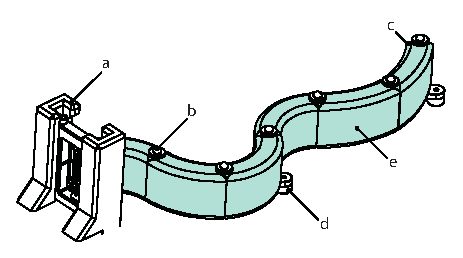
\includegraphics[width=0.9\columnwidth]{figures/manipulators/ribbed_manipulator}
            \caption{}
            \label{fig:ribbed_manipulator_design}
        \end{subfigure}\\
        \begin{subfigure}[b]{\columnwidth}
            \centering
            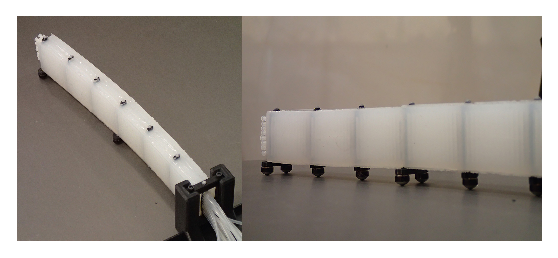
\includegraphics[width=0.9\columnwidth]{figures/manipulators/ribbed_manipulator_real}
            \caption{}
            \label{fig:ribbed_manipulator_real}
        \end{subfigure}%
        \caption[A ribbed soft manipulator prototype.]{A ribbed soft manipulator prototype. (\textbf{a}) The arm is composed of homogeneous and independently actuated ribbed segments (e). The base of the arm's first segment is fixed (a) and the end of its last segment is the end-effector (c). Markers (b) identify the endpoints of each segment and ball transfers (d) mitigate friction. (\textbf{b}) Photographs of the ribbed manipulator prototype.}
\end{figure}

\subsection{Cylindrical}
\label{subsec:Manipulators, Cylindrical}
We can also compose a manipulator from cylindrical fluidic elastomer segments, as shown in Figure~\ref{fig:cylindrical_manipulator} and initially developed in \citet{marchese2014whole}.
Just as in the ribbed composition, cylindrical segments are joined end-to-end.
Here, fluid transmission lines are passed through the manipulator's hollow center.
This feature not only facilitates segment concatenation, but also allows for modular composition of a manipulator, because transmission lines are not permanently embedded within the elastomer.
Additionally, this manipulator type is only composed of soft silicone rubber as there is no inextensible constraint.
No other materials are used, except for the attached ball transfers to mitigate ground friction.
\begin{figure}[htb]
\centering
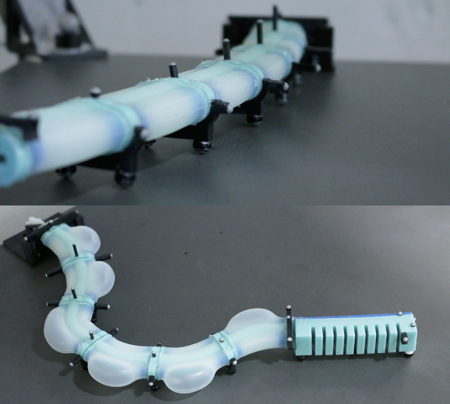
\includegraphics[width=\columnwidth]{Figures/manipulators/cylindrical_manipulator_real}
\caption[A cylindrical planar soft manipulator prototype.]{A planar cylindrical soft manipulator prototype with and without a pleated finger-like gripper.} \label{fig:cylindrical_manipulator}
\end{figure}

Additionally, using four actuated channels per body segment, we have created a multi-segment spatial cylindrical manipulator in \citet{marchese2015design}. This enables three-dimensional end-effector positioning and is shown in Figure~\ref{fig:spatial_cylindrical_manipulator}.

\begin{figure}[htb]
\centering

\includegraphics[width=0.3\columnwidth]{Figures/manipulators/CshapeTight.eps}
\caption[A cylindrical spatial soft manipulator prototype.]{A spatial cylindrical soft manipulator prototype.} \label{fig:spatial_cylindrical_manipulator}
\end{figure}

\subsection{Pleated}
\label{subsec:Manipulators, Pleated}
A manipulator can also be composed from pleated fluidic elastomer segments, as shown in Figure~\ref{fig:pleated_manipulator}.
Just as in the ribbed and cylindrical composition, pleated segments are joined end-to-end.
The fluid transmission lines are passed through along the central axis of the segments.
A supportive hollow profile can be added to combine two segments.
This pleated design allows for modular composition of a manipulator, because transmission lines are not permanently embedded within the elastomer.
Additionally, this type of manipulator is, like the cylindrical manipulator, composed entirely of soft silicone rubber.
\begin{figure}[htb]
\centering
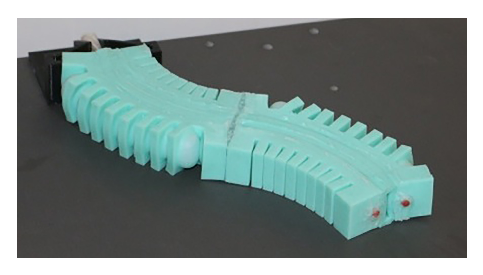
\includegraphics[width=\columnwidth]{Figures/manipulators/pleated_manipulator_real}
\caption[A pleated soft manipulator prototype.]{A pleated soft manipulator prototype, composed of two segments with two degrees of freedom each.}
\label{fig:pleated_manipulator}
\end{figure} 